\chapter{State of the art}

In questo capitolo saranno inizialmente esposti i concetti teorici alla base dell'applicazione 
sviluppata: dagli algoritmi più comuni per la \textbf{Face Detection} 
ad un'introduzione al \textbf{Machine Learning} per finire
poi con elementi di \textbf{Programmazione Lineare Multiobiettivo}.

Verranno quindi analizzati precedenti progetti che hanno affrontato le stesse problematiche.

\section{Face Detection}

La Face Detection è una tecnologia
che permette di localizzare ed estrarre da un'immagine la regione contenente un 
volto \cite{Datta2015}; ha oggigiorno diverse applicazioni ed utilizzi, dal 
video coding al content-based image retrieval. 

\begin{figure}
    \begin{small}
        \begin{center}
            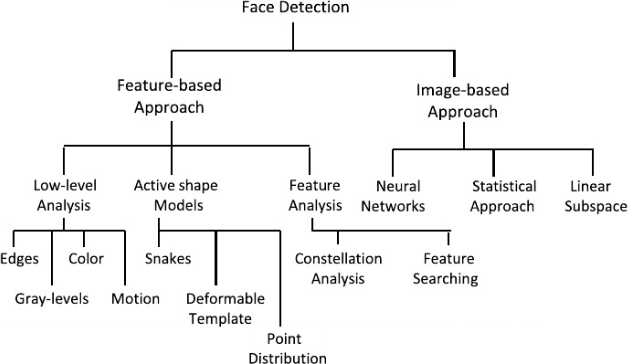
\includegraphics[width=0.95\textwidth]{face_detection_techniques.png}
        \end{center}
        \caption{Diversi approcci alla face detection}
        \label{fig:face_detection_approaches}
    \end{small}
\end{figure}

\subsection{Problematiche comuni}

Le sfide che una tecnica di face detection si trova ad affrontare sono solitamente 
(\cite{Datta2015}):

\begin{itemize}
    \item \textbf{Occlusione}. Spesso parte dei volti sono nascosti da oggetti e/o 
        altri volti
    \item \textbf{Espressioni}. L'aspetto dei volti è fortemente influenzato 
        dall'espressione della persona.
    \item \textbf{Posa}. La posizione da cui è scattata l'immagine influenza la 
        prospettiva del volto (\ref{fig:fd_problem}).
    \item \textbf{Luminosità}. Livelli di luminosità eccessivi o troppo bassi 
        impediscono di ricoscere contorni e linee del viso.
\end{itemize}

\begin{figure}
    \begin{small}
        \begin{center}
            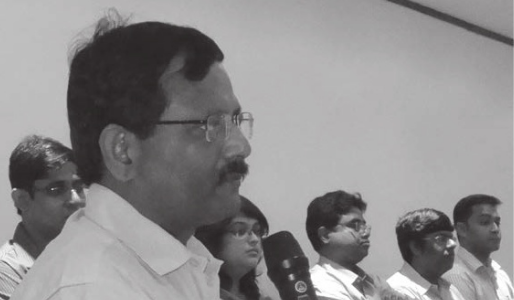
\includegraphics[width=0.50\textwidth]{face_detection_situation.png}
        \end{center}
        \caption{Un classico esempio di problema di face detection}
        \label{fig:fd_problem}
    \end{small}
\end{figure}

\subsection{Approcci feature-based}

In un periodo di ricerca che coinvolge circa gli ultimi trenta anni sono state 
usati diversi approcci che permettessero di sviluppare tecniche di face detection
(\ref{fig:face_detection_approaches}), dividendosi principalmente in due categorie: 
\textbf{Feature-based} e \textbf{Image-based}.

Nei primi vengono solitamente estratte le feature di un volto da 
un'immagine (come ad esempio occhi, labbra, sopracciglia) per poi verificare, 
attraverso la relazione che persiste tra di loro, la presenza di un volto.

All'interno di questa categoria possono essere indivuate ulteriori distinzioni
(\cite{Datta2015}, 2.2):

\begin{itemize}
    \item \textbf{Low Level Analysis}. Feature vengono estratte basandosi sulle 
        proprietà dei pixel come ad esempio colore o valore nella scala di grigi.
    \item \textbf{Feature Analysis}. Vengono sfruttate le proprietà geometrice 
        del volto per cercare di localizzare ed individuare le diverse parti del viso.
    \item \textbf{Active shape models}. Questi modelli, che vanno da \textit{snakes}
        ai PDM (point-distributed models) sono usati per l'estrazione di feature 
        complesse e per tracciare le iridi degli occhi e le labbra.  
\end{itemize}

\subsection{Algoritmo Viola-Jones per la Face Detection}

Invece tra gli svariati approcci \textbf{Image-based} uno che ha avuto particolare successo, soprattutto per la 
velocità di calcolo che permette il suo utilizzo in applicazioni che utilizzano grandi 
moli e flussi di immagini, è l'algoritmo Viola-Jones.

\medskip

Esso fa uso di Haar functions per il l'individuazione delle features, i.e. 
si basa sul calcolo della somma e differenza di pixel in particolari rettangoli 
\cite{Viola2004}, come mostrato in \ref{fig:haar}.

Il calcolo viene enormemente velocizzato attraverso le \textit{integral images}, 
immagini in cui il valore dei pixel è pari alla somma dei pixel in alto a sinistra, i.e.

\begin{equation}
    ii(x,y) = \sum_{x'\leq x, y' \leq y}^{} i(x', y')
    \label{eq:}
\end{equation}

con $ii(x,y)$ il valore del pixel nella \textit{integral image} e $i(x',y')$ 
il valore nell'immagine originale.

\begin{figure}
    \begin{small}
        \begin{center}
            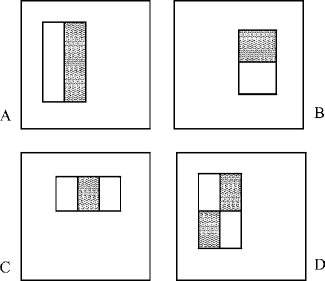
\includegraphics[width=0.40\textwidth]{haar_example.png}
        \end{center}
        \caption{Al valore dei pixel nella regione bianca viene sottratto il valore nella regione scura}
        \label{fig:haar}
    \end{small}
\end{figure}

\medskip

Tali \textit{Haar functions} vengono usate quindi da \textbf{classificatori}, 
delle funzioni che mappano un'osservazione (in questo caso un insieme di pixel) su un un set finito di valori, 
in questo caso \cite{Wang2014}
$f:$\Rset$^d\rightarrow \{-1, 1\}$.

Attraverso un Ada Boosting questi singoli ed imprecisi classificatori vengono combinati tra di loro
per ottenere un classificatore "forte" che risulta essere molto più accurato \cite{Schapire2013} dei singoli.

Dato un esempio da classificare $x$, l'esito della classificazione "forte" è pari a 

\begin{equation}
    F(x) = \sum_{t=1}^{T} \alpha_t h_t(x)
    \label{eq:}
\end{equation}

con $h_t(x)$ classificatore "debole" a cui corrisponde un peso "di voto" pari a $\alpha_t$:
il risultato è quindi ottenuto come la maggioranza pesata delle classificazioni deboli.

\medskip

Il rendimento può essere ulteriormente migliorato con l'utilizzo di classificatori a cascata 
(\ref{fig:cascade}). Un classificatore a cascata è costituito da diversi \textit{stages}, 
ognuno contenente uno classificatore "forte", ciascuno dei quali determina se la finestra in 
input non contiente sicuramente un volto oppure potrebbe. Quando viene predetta l'assenza 
certa di un viso l'immagine viene scartata, altrimenti è passata allo \textit{stage} successivo 
\cite{Datta2015}.

\begin{figure}
    \begin{small}
        \begin{center}
            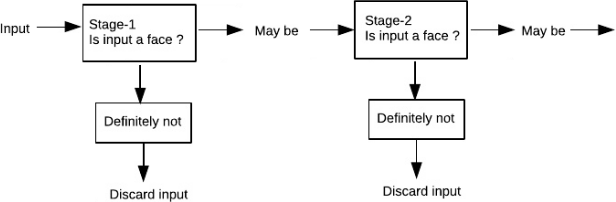
\includegraphics[width=0.95\textwidth]{cascade.png}
        \end{center}
        \caption{Struttura dei classificatori a cascata}
        \label{fig:cascade}
    \end{small}
\end{figure}

